\section{Results}\mbox {} \
\label{sec:results}

We demonstrate that our attacks are highly effective against the state-of-the-art ReCAPTCHA service by Google. Together with the user agent vulnerability that we uncovered and using Google's Cloud Speech API, our attacks are most effective against Google's reCAPTCHA than other existing CAPTCHA providers as shown in Fig.3. This high accuracy was based on little or no background noise in ReCAPTCHA's audio and highly efficient speech recognition systems. Although the vulnerability has since been fixed, the audio challenges remain very simple to crack.  \newline

We found that the US accent solved the challenges with a higher accuracy than the UK accent, with the exception of Securimage and Captchas.net where we had higher accuracy with the UK accent solver from Google's Cloud Speech API. We also found that IBM Watson's Speech to Text API was the next best solver for ReCAPTCHA's audio challenges. 0The increase in time for the other services was due to the background noise and more complex challenges than ReCAPTCHA.\newline

We also show that our attack was least effective against Securimage, which uses background noise to mask the audio. We would like to mention here that Securimage is an open source system that provides the source files, including the noise files which would allow the attacker to easily filter out the noise as it is known beforehand. We consider this to be an important future work.

\begin{figure}[t]
   \centering
   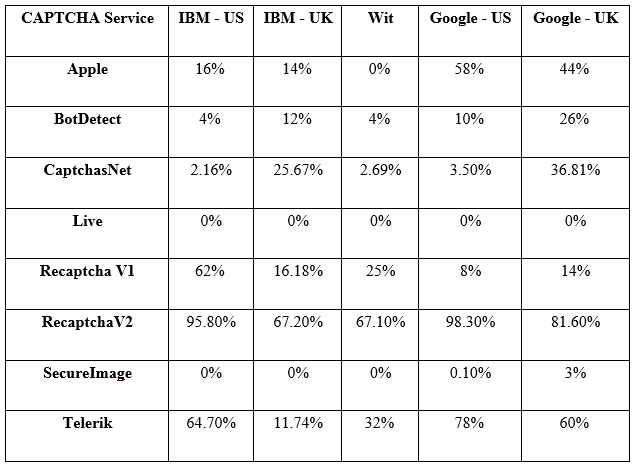
\includegraphics[width=\columnwidth]{figures/res1.png}.
   \caption{Results: Accuracy of solving various CAPTCHAs using the different solvers.}
   \label{fig:example}
\end{figure}
